%!TEX root = <main.tex>
\section{Introduction}
Deep Convolution Neural Networks (CNNs) \cite{alexnet, vggnet, resnet, inception} have revolutionized the computer vision field with even surpassing human level accuracy in some of the image recognition challenges such as ImageNet~\cite{imagenet}.
% Many of these successful pre-trained CNNs from computer vision challenges have been successfully re-purposed to be used in other real-world image recognition tasks using a paradigm called \textit{transfer learning} \cite{transfer-learning-factors}.
% In transfer learning, instead of training a CNN from scratch, one uses a pre-trained Deep CNN, e.g., ImageNet trained VGG, and fine tune it for the target problem using the target training dataset.
% This approach avoids the need for a large training datasets, computational power, and time which is otherwise a bottleneck for training a CNN from scratch.
As a result, there is wide adoption of Deep CNN technology in a variety of real-world image recognition tasks in several domains including healthcare \cite{kermany2018identifying, islam2017abnormality}, agriculture \cite{mohanty2016using}, security \cite{arbabzadah2016identifying}, and sociology \cite{wang2017deep}.
Remarkably, United States Food and Drug Administration Agency (US FDA) has already approved the use of Deep CNN based technologies for identifying diabetic retinopathy, an eye disease found in adults with diabetes \cite{fdaretinopathy}.
It is expected that this kind of decision support systems will help the human radiologists in fulfilling their workloads efficiently, such as functioning as a cross-checker for the manual decisions and also to prioritize potential sever cases for manual inspection, and provide a remedy to the shortage of qualified radiologists globally \cite{radiologistshortage}.

\begin{figure}[t]
  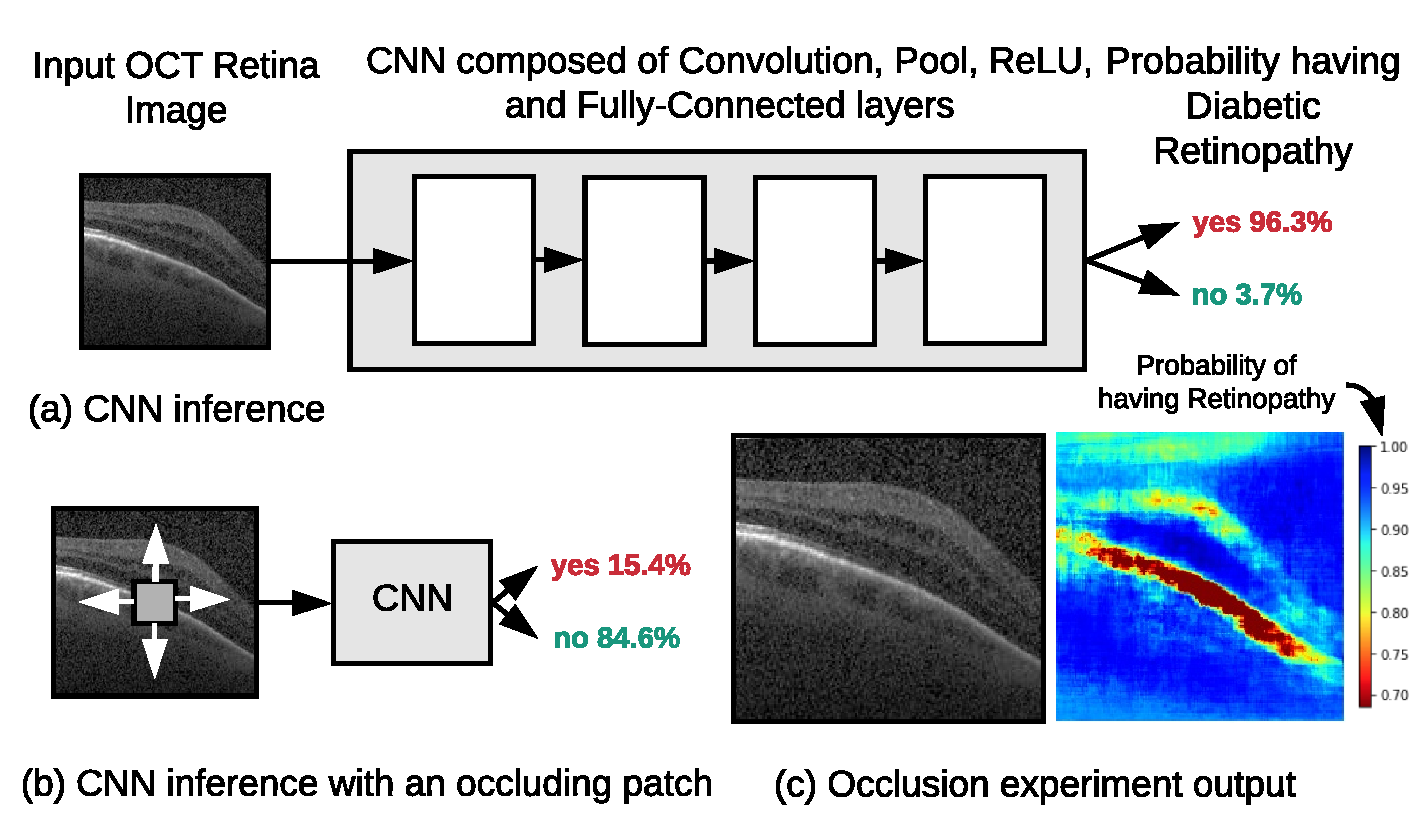
\includegraphics[width=\columnwidth]{./images/krypton_overview}
  \caption{(a) Using CNNs for predicting Diabetic Retinopathy from OCT images. (b) Occluding parts of the OCT image changes the predicted probability for the disease. (c) By changing the position of the occlusion patch a sensitivity heat map is produced.}
  \label{fig:krypton_overview}
\end{figure}

Despite their many success stories, one of the major criticisms for deep CNNs and deep neural networks, in general, is the black-box nature of how they make predictions.
In order to apply deep CNN based techniques in critical applications such as healthcare, the decisions should be explainable so that the practitioners can use their human judgment to decide whether to rely on those predictions or not \cite{jung2017deep}.
One of the widely used approach for explaining CNN predictions is the \textit{occlusion based explanations} (OBE) approach \cite{zeiler2014visualizing}.
In OBE experiments a square patch, usually of black or gray color, is used to occlude parts of the image and record the change in the predicted label probability as shown in Figure~\ref{fig:krypton_overview} (b).
By changing the position of the occlusion patch a sensitivity heat map for the predicted label, similar to the one shown in Figure~\ref{fig:krypton_overview} (c), can be generated.
Using this heat map, the regions in the image which are highly sensitive (or highly contributing) to the predicted class can be identified (corresponds to red color regions in the sensitivity heat map shown in Figure~\ref{fig:krypton_overview} (c)).
This localization of highly sensitive regions then enables the practitioners to get an intuition of the the prediction process of the deep CNN.

% If the occlusion experiment is performed in interactive mode, the human operator has the option of picking the occlusion patch positions by marking a region on a visual interface.
% For example, if the scenario shown in Figure \ref{fig:krypton_overview} is performed in interactive mode, the human operator who understands OCT images will start evaluating the image from the central region where she expects the pathological region to most likely to be.
% In the non-interactive mode, which is also the most common mode of performing occlusion experiments due to the high runtimes which are not amenable for interactive performance, the heat map values are evaluated for all possible occlusion patch positions.


% \textbf{\textit{Example:}} Consider a radiologist who is examining Optical Coherence Tomography (OCT) images of the retina to identify potential diabetic retinopathy patients.
% The radiologist is recently given access to a Deep CNN based clinical decision support system (CDSS) to identify potential images with diabetic retinopathy. 
% It predicts the probability whether a retina image depicts a diabetic retinopathy case.
% She uses the CDSS for two main purposes: 1) as a cross checker while manually inspecting the retinal images, and 2) to prioritize potentially sever cases from a backlog of retina images.
% In both situations in addition to predicting the existence of the disease, she would like to have an explanation for the basis on which the CDSS makes the prediction, using the occlusion based explainability approach, to decide whether the pathological regions identified by the CDSS are correct and to ultimately whether to rely on the CDSS decision. Similar examples arise in number of other heal care applications such as chest X-ray examination for identifying pneumonia cases and X-ray based child bone age assessment.

Alas, this approach creates a new bottleneck: OBE experiments are highly compute intensive and time consuming due to the large number of re-inference requests that needs to be performed.
The current approach to perform OBE experiments is to generate a large number of modified versions of the original image with each image corresponding to a specific occlusion patch position and perform CNN inference for those images using a tool like PyTorch \cite{ketkar2017introduction}.
In extreme cases this approach can generate more than 500,000 different images and can take up to more than one hour to complete, even by using a GPU~\cite{zintgraf2017visualizing}.
Such long execution times hinders the data scientist's ability to analyze CNN predictions and also reduces their productivity.

\textit{In this work we apply database inspired optimizations to the OBE workload to reduce both the computational cost and the runtime}.
Our work is motivated by the simple yet crucial observation: different occluded instances of the original image are \textit{not} independent -- when performing CNN inference corresponding to each individual occluded image significant portion of redundant computation can be avoided.
This observation leads us to a classical database systems-style concern: \textit{view maintenance}.
In database parlance, the current approach of performing CNN inference for each occluded instance of the image independently can be considered as a form of \textit{complete view maintenance}, where a ``view'' is a layer of CNN features.
This approach wastes runtimes due redundancy in CNN inference computations across occluded instances of the original image. 

We formalize the dataflow of the layers of a CNN and create a novel and comprehensive algebraic framework for \textit{incremental inference} of CNN which combines \textit{incremental view maintenance} (IVM) \cite{chirkova2012materialized,gupta1995maintenance,levy1995answering} with \textit{multi-query optimization} (MQO) to avoid computational redundancy across re-inference requests.
Using our algebraic framework we theoretically characterize how much speedups one can expect from incremental inference for different CNN models.
To the best of our knowledge, this is the  first known instance of fusing an IVM-style techniques with an MQO-style technique for optimizing CNN inference.

We then introduce \textit{approximate inference} optimizations that exploit a capability of human perception: tolerance of some degradation in visual quality of the heat maps.
We build upon our incremental inference optimizations to create two novel approximate inference optimizations that trade off the quality of the generated heat map in a user tunable manner to accelerate OBE.
Our approximate inference optimizations are inspired by the \textit{approximate query processing} (AQP) techniques used for answering statistical analytical queries in RDBMs.
However, our focus here is on minimizing the perceivable differences of the generated heat maps where as in traditional AQP the focus is on minimizing the statistical error.
We also combine AQP and MQO style techniques to reduce OBE runtime.


% This will also make occlusion experiments more amenable for interactive diagnosis of CNN predictions.

% Due to the overlapping nature of how the Convolution kernel operates (details to follow in Section \ref{sec:preliminaries}), the size of the modified patch will start growing as it progresses through more layers in a CNN and the amount of redundant computations will reduce.
% However, at deeper layers, the effect over the patch coordinates which are radially further away from the center of the occlusion patch position will be diminishing.
% Our second optimization is based on this observation where we apply a form of \textit{approximate inference} which applies a threshold to limit the growth of the updating patch. 
% By applying propagation thresholds, a significant amount of computation redundancy can be retained.
% We refer to this optimization as \textit{projective field thresholding}.

% The third optimization is also a form of \textit{approximate inference} which is applicable only in the context of non-interactive mode.
% In most occlusion experiment use cases, such as in medical imaging, the object or pathological region of interest is contained in a relatively small region of the image.
% In such situations, it is unnecessary to inspect the original image at the same high resolution of striding the occluding patch few pixels at a time, at all possible occlusion patch positions.
% In this approach first, a low-resolution heat map is generated using a larger stride value with a relatively low computational cost.
% Only the interesting regions will be then inspected further with a smaller stride to produce a higher resolution output.
% In the interactive mode, as the human operator will be actively picking a set of occlusion patch positions for the system to evaluate this optimization will not be applicable.
% We refer to this optimization as \textit{adaptive drill-down}.

% Unlike the \textit{incremental inference} approach which is exact, \textit{projective field thresholding} and \textit{adaptive drill-down} are approximate approaches. They essentially trade-off accuracy of the generated sensitivity heat map compared to the original, in favor of faster execution.
% These changes in accuracy in the generated heat map can be visible all the way from quality differences which are almost indistinguishable to the human eye to drastic structural differences, depending on the level of approximation.
% This opens up an interesting trade-off space of quality/accuracy versus runtime. \system~ provides user configurable tuning parameters for easily picking an operational point on this quality-runtime trade-off space.

We prototype our ideas as a system we call \system~ on top of PyTorch deep learning toolkit by adding custom implementations for incremental and approximate inference operations.
It currently supports VGG16, ResNet18, and InceptionV3 both on CPU and GPU environments, which are three widely used Deep CNN architectures.
We evaluate our system on three real-world datasets, 1) retinal optical coherence tomography dataset (OCT), 2) chest X-Ray, and 3) more generic ImageNet dataset.
While we have implemented \system~ on top of PyTorch toolkit, our work is largely orthogonal to the choice of the deep learning toolkit; one could replace PyTorch with TensorFlow, Caffe2, CNTK, MXNet, or implement from scratch using C/CUDA and still benefit from our optimizations.
Overall, this paper makes the following contributions:

\begin{itemize}
	\item To the best of our knowledge, this is the first paper to study the incremental inference and approximate inference optimizations for the OBE workload from a systems standpoint.

	\item We develop a comprehensive algebraic framework for incremental inference of CNN which combines IVM with MQO to avoid computational redundancy across re-inference requests.

	\item We also introduce two approximate inference optimizations that exploit the characteristics of human perception to further reduce runtimes of the OBE workload.

	\item Using a prototype system call \system, we present an extensive empirical evaluation of the benefits of our optimizations. Overall, \system~  can result in speedups up to 5x (14x) to produce exact (approximate) heat maps.

\end{itemize}

\vspace{2mm}
\noindent \textbf{Outline.} The rest of this paper is organized as follows.
Section 2 formally define the problem, explains our assumptions, and formalizes the dataflow of layers of a CNN.
Section 3 provides a theoretical characterization of potential speedups for different CNN models and presents our novel algebraic framework for performing incremental inference for OBE.
Section 4 presents our approximate inference optimizations.
Section 5 presents the experimental evaluation.
We discuss other related work in Section 6 and conclude in Section 7.
